This section describe all the experiments that we have done  using the different algorithms and the different robots setups too.

\subsection{Snake Robot}
The snake robot is a highly articulated robot with a number of joints connected to each other serially, developed at the Biorobotics laboratory at Carnegie Mellon University. An example of this robot is shown in Fig. \ref{fig:snake}. A video of the snake experiments that we did can be reached at https://youtu.be/Cy4igTHlHW4 .
\begin{figure}[t]\label{fig:snake}
	\centering
	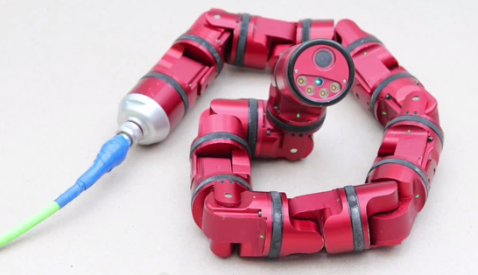
\includegraphics[width=0.7\linewidth]{figures/snake}
	\caption{The snake robot of the Biorobotics Laboratory at CMU, that we used to test and compare how well the ORB and LSD SLAM algorithms work on highly dynamics robots. }
	\label{fig:snake}
\end{figure}


\begin{figure}[t]\label{fig:goat}
	\centering
	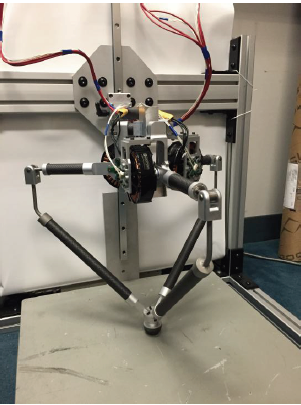
\includegraphics[width=0.7\linewidth]{figures/goat}
	\caption{The Goat Leg (jumping monopod) that we used as one interesting platform to test the SLAM algorithms}
	\label{fig:goat}
\end{figure}

\subsection{GOAT: Jumping Monopod}
The Goat is a jumping monopod developed by the Biorobotics laboratory at Carnegie Mellon University. It has a Gearless Omni-directional Acceleration-vectoring Topology, which is a novel leg design aimed at surpassing all current leg designs in terms of 3D agility. The GOAT leg is modular in that it can be configured with various drive motors and gear-trains for
either DD or QDD. Additionally, the leg can be used in various legged robot morphologies including
monopod, biped, tripod and quadruped. Due to the highly dynamic nature of this robot, we aimed to test and evaluate the state of the art SLAM algorithms on it cause these algorithms migt not behave as well as on mobile robots for example, due to the very fast motion of this robot and the huge shaking of the image while the robot is jumping. A video of the GOAT can be found at https://www.youtube.com/watch?v=n319xVomJTQ.
